\chapter{Advanced Class Modeling}
\index{Advanced Class Modeling}
\label{Chapter::AdvancedClassModeling}



\section{Exercises}
\noindent\rule{\textwidth}{0.4pt} % Line


\subsection{Exercise 3.1}
\paragraph{Part 1}
\begin{itemize}
    \item The \textbf{Buffer} is associated with both the \textbf{Sheet} and \textbf{Selection} classes, with a multiplicity of 0..1, meaning it is optional.
    \item The \textbf{Selection} class is also optional, with the same multiplicity (0..1) and is linked to the \textbf{Sheet}.
    \item The \textbf{Sheet} class is the central element, connected to the \textbf{Buffer}, \textbf{Selection}, \textbf{Line}, and \textbf{Box} classes, each with a multiplicity of 0..1, meaning a \textbf{Sheet} can have at most one instance of each.
    \item The \textbf{Line} class is associated with the \textbf{Sheet} (multiplicity 0..1) and must have one \textbf{LineSegment} (multiplicity 1).
    \item The \textbf{LineSegment} class is linked to the \textbf{Point} class with a multiplicity of 1..2, meaning it must have one or two \textbf{Points}.
    \item The \textbf{Point} class represents the points that define the geometry of a \textbf{LineSegment}.
\end{itemize}

\paragraph{Part 2}
\begin{figure}[H]
    \centering
    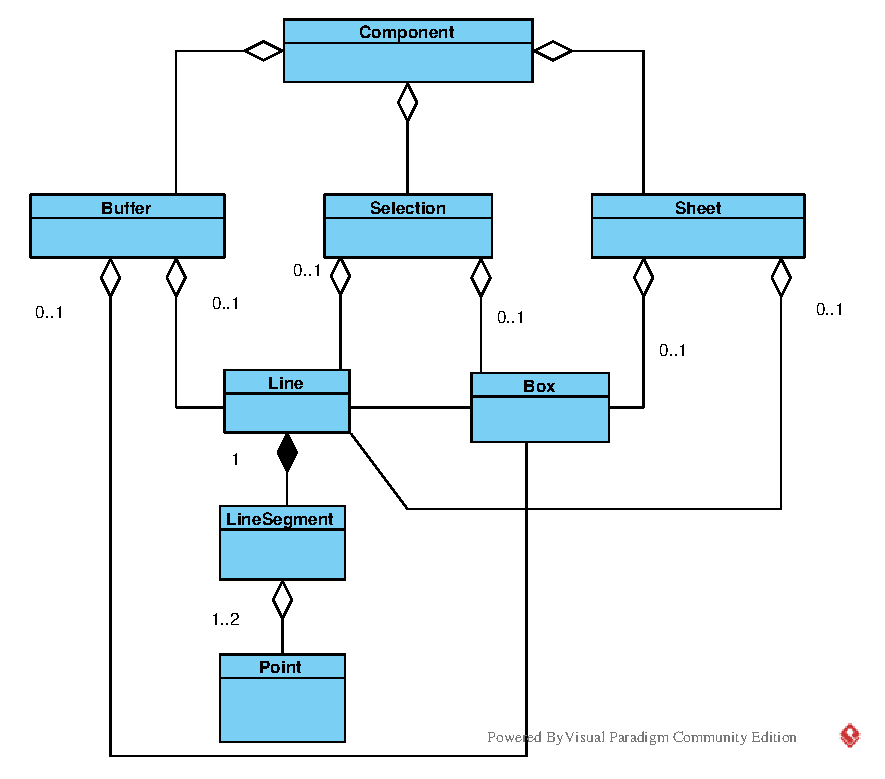
\includegraphics[width=\textwidth]{images/EPS/Exercise-1_Part-2.eps}
    \caption{Revised simple editor class hierarchy}
    \label{fig:Exercise-1_Part-2}
\end{figure}

\subparagraph{Merits of the Revision}
\begin{itemize}
    \item \textbf{Simplified Maintenance:} Having a base class like Component reduces redundancy, as the common logic related to managing collections of lines and boxes is encapsulated in a single place.
    \item \textbf{Enforcement of Constraints:} This revision enforces the rule that a Line or Box can only belong to one Component (either Buffer, Selection, or Sheet), preventing any ambiguity in ownership.
    \item \textbf{Flexible Extension:} If, in the future, more types of collections (other than buffer, selection, or sheet) need to be added, they can simply inherit from Component.
    \item This revised diagram would address the problem stated in part 2 by clearly enforcing the "exactly one" rule, while also making the class structure more flexible and easier to extend.
\end{itemize}

\noindent\rule{\textwidth}{0.4pt} % Line


\subsection{Exercise 3.2}
\begin{figure}[H]
    \centering
    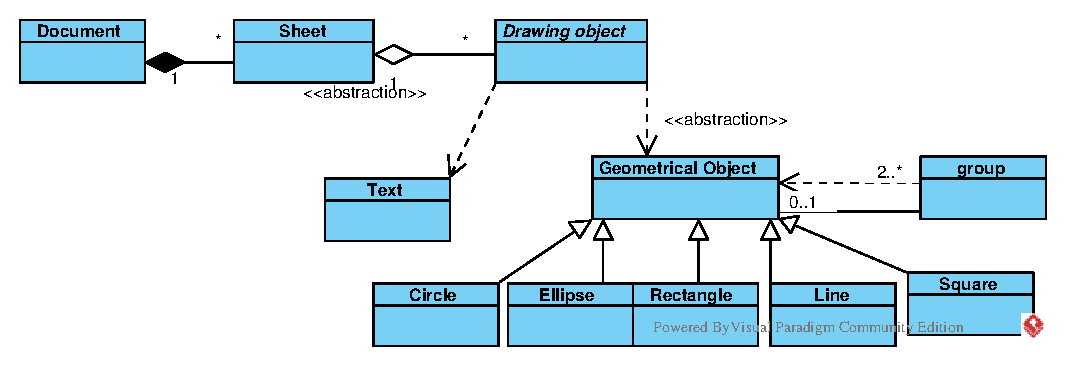
\includegraphics[width=\textwidth]{images/EPS/graphicalDocumentEditor.eps}
    \caption{Class diagram for a graphical Document editor}
    \label{fig:GraphicalDocumentEditor}
\end{figure}

\noindent\rule{\textwidth}{0.4pt} % Line


\subsection{Exercise 3.3}
\begin{figure}[H]
    \centering
    \includegraphics[width=\textwidth]{images/EPS/ElectricalMotors.eps}
    \caption{Electrical motors class diagram}
    \label{fig:ElectricalMotors}
\end{figure}
Multiple inheritance was used for the electric motor, as it can be generalized into either a type of alternating current or direct current.
\begin{figure}[H]
    \centering
    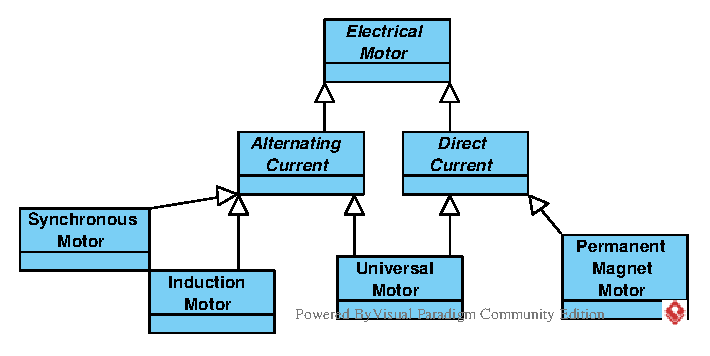
\includegraphics[width=\textwidth]{images/EPS/ElectricalMotorsabstracted.eps}
    \caption{Revised Electrical motors class diagram}
    \label{fig:RevisedElectricalMotors}
\end{figure}
By abstracting the AC and DC current classes, we are able to allow each individual motor to be derived from a different type of current.

\noindent\rule{\textwidth}{0.4pt} % Line


\subsection{Exercise 3.4}
\url{https://github.com/ryry91021/ssw345-labs/blob/main/AdvancedClassModelingLab/wk3StateMachines.py}
\begin{figure}[H]
    \centering
    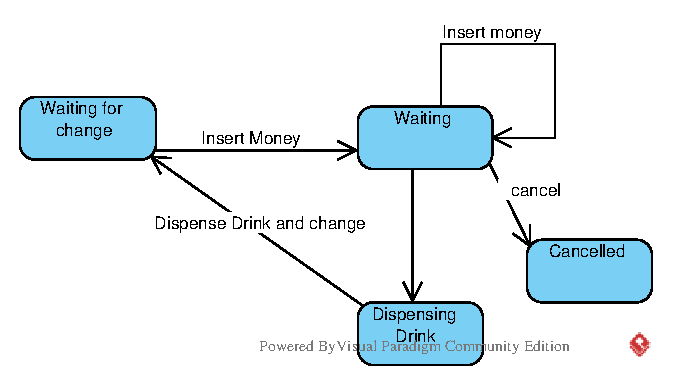
\includegraphics[width=\textwidth]{images/EPS/stateMachineVending.eps}
    \caption{Vending machine class diagram}
    \label{fig:Vending Machine}
\end{figure}

\noindent\rule{\textwidth}{0.4pt} % Line


\subsection{Exercise 3.5}

% PART 1: CRC Cards
\paragraph*{Part 1: CRC Cards}
\begin{table}[H]
    \centering
    \begin{tabular}{@{}lll@{}}
        \toprule
        \textbf{Class}       & \textbf{Responsibilities}                                      & \textbf{Collaborations}               \\ \midrule
        Student              & \begin{tabular}[c]{@{}l@{}}- Manage student info\\ - Select transportation\\ - Go to class\end{tabular} & \begin{tabular}[c]{@{}l@{}}- Transportation\\ - Class\end{tabular}                  \\
        Transportation       & \begin{tabular}[c]{@{}l@{}}- Manage transport modes\\ - Provide transport info\end{tabular}                    & \begin{tabular}[c]{@{}l@{}}- Student\\ - Bike\\ - Shoes\end{tabular}                   \\
        Bike                 & \begin{tabular}[c]{@{}l@{}}- Represent bike attributes\\ - Facilitate riding to class\end{tabular}              & \begin{tabular}[c]{@{}l@{}}- Transportation\\ - Student\end{tabular}                \\
        Shoes                & \begin{tabular}[c]{@{}l@{}}- Represent shoe attributes\\ - Facilitate walking to class\end{tabular}             & \begin{tabular}[c]{@{}l@{}}- Transportation\\ - Student\end{tabular}                \\
        Class                & \begin{tabular}[c]{@{}l@{}}- Manage class info\\ - Schedule class\end{tabular}                                    & \begin{tabular}[c]{@{}l@{}}- Student\end{tabular}                                \\ \bottomrule
    \end{tabular}
    \caption{CRC Cards/Table for Student Transportation Simulation}
\end{table}

The CRC card creation process began by identifying the key classes present in the user story, specifically focusing on John and Maria's actions and interactions. The main classes came from the characters and their transportation methods: Student, Transportation, Bike, Shoes, and Class. Each class was analyzed to determine its responsibilities and correlation with other classes. For instance, the Student class was responsible for managing student information and selecting transportation, while the Transportation class served as a parent for specific transport methods. This initial analysis helped clarify the structure of the system and laid the groundwork for the subsequent diagrams.

\vspace{1cm} % Vertical space

% PART 2: Use Case Diagram
\paragraph*{Part 2: Use Case Diagram}
\begin{figure}[H]
    \centering
    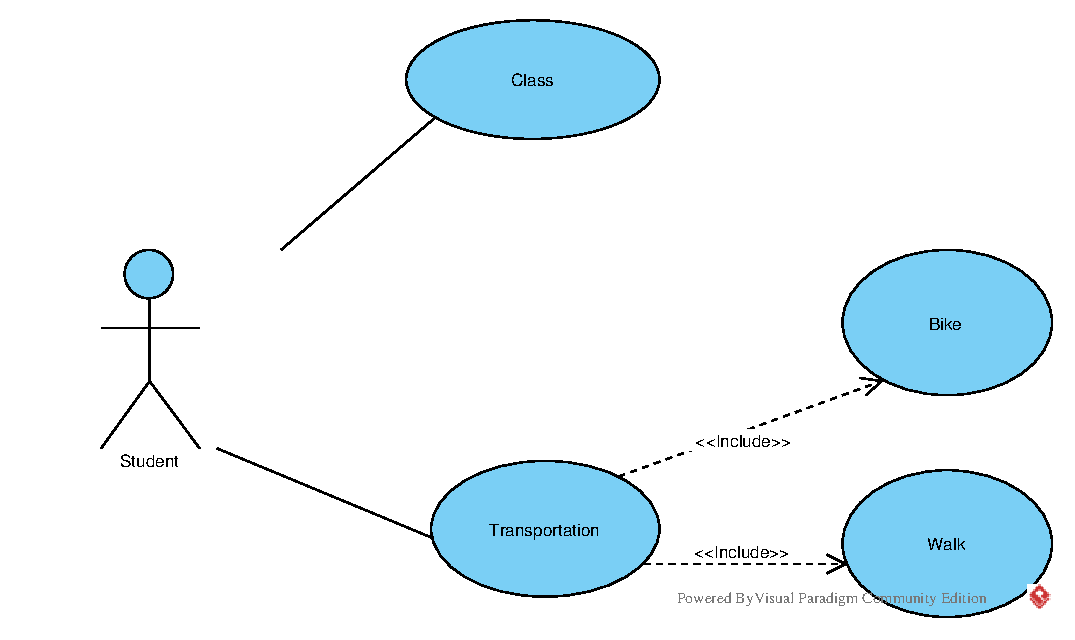
\includegraphics[width=\textwidth]{images/EPS/ex3-5_useCase.eps}
    \caption{Use Case Diagram for Students}
    \label{fig:ex3-5_useCase}
\end{figure}

When constructing the use case diagram, I aimed to capture the interactions between the Student and their actions in relation to transportation and class attendance. The main use cases were identified as selecting transportation, attending class, riding a bike, and walking to class. I chose to use inclusion relationships to show that selecting transportation leads to either riding a bike or walking to class. This diagram succinctly represents the students' journey from selecting how to get to class to actually attending the class. The use case diagram effectively visualizes the system's functionality from the user's perspective, providing a clear view of the processes involved.

\vspace{1cm} % Vertical space

% PART 3: Object Diagram
\paragraph*{Part 3: Object Diagram}
\begin{figure}[H]
    \centering
    \includegraphics[width=\textwidth]{images/EPS/ex3-5_part3.eps}
    \caption{Object Diagram: Student Transportation Scenario}
    \label{fig:ex3-5_part3}
\end{figure}

The object diagram was created as a concrete snapshot of the system based on the previously defined classes and their relationships. I focused on instantiating the main objects, such as John, Maria, Bike, Shoes, and Class, to reflect the specific scenario outlined in the user story. The associations among these objects were carefully mapped to illustrate how John uses a bike and Maria uses shoes to reach the same class. This diagram highlights the real-time interaction between the objects and provides insight into how the system behaves during a specific instance. It serves as a bridge between the abstract class structures and the practical, real-world scenario presented in the user story.

\vspace{1cm} % Vertical space

% PART 4: Class Diagram
\paragraph*{Part 4: Class Diagram}
\begin{figure}[H]
    \centering
    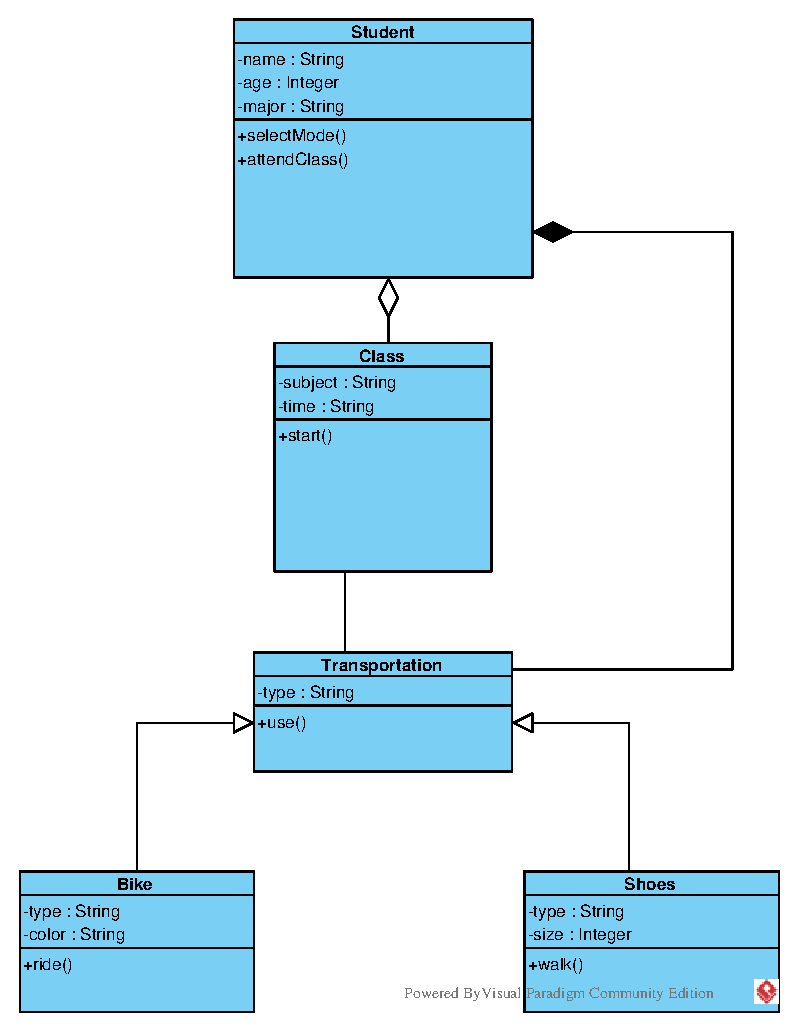
\includegraphics[width=\textwidth]{images/EPS/ex3-5_part4.eps}
    \caption{Class Diagram: Student Transportation System}
    \label{fig:ex3-5_part4}
\end{figure}

In developing the class diagram, I synthesized information from the previous diagrams and refined the relationships between the classes. I recognized that Transportation could serve as an abstract class with sub-classes for Bike and Shoes, reflecting the generalization of transportation modes. I included attributes and methods for each class to provide a comprehensive view of their functionality. The relationships were explicitly defined, using multiplicities to clarify the number of instances involved, such as a Student having exactly one Transportation method and a Class potentially having multiple Students. This diagram serves as a more structured representation of the system's architecture, emphasizing the organization and hierarchy of classes while highlighting their interactions.

\vspace{1cm} % Vertical space

\noindent\rule{\textwidth}{0.4pt} % Line


\subsection{Exercise 3.6}

\vspace{1em} % Adds space before the figures

\begin{figure}[H]
    \centering
    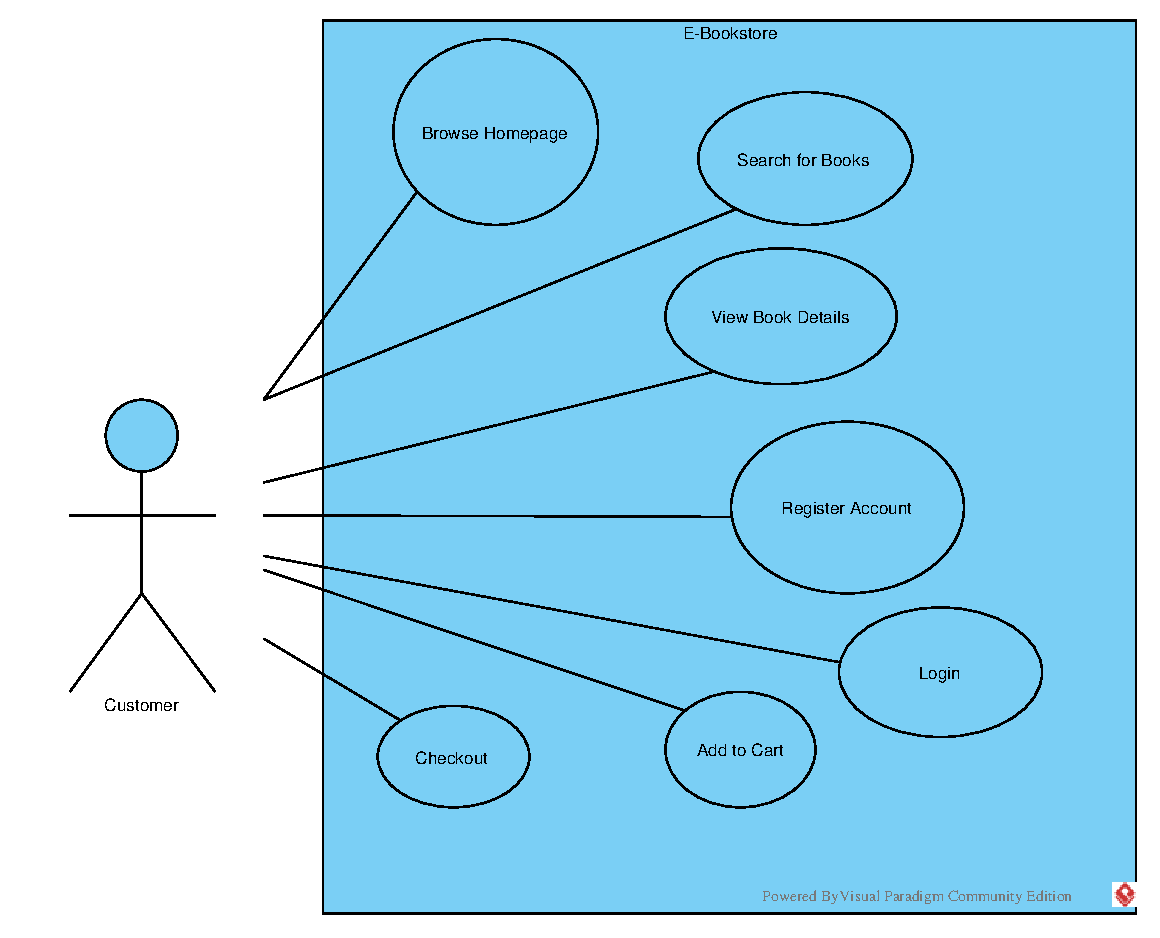
\includegraphics[width=\textwidth]{images/EPS/q6-part1.eps}
    \caption{Use Case Diagram for E-Bookstore}
    \label{fig:q6-part1}
\end{figure}

\vspace{1em} % Adds space between figures
\begin{figure}[H]
    \centering
    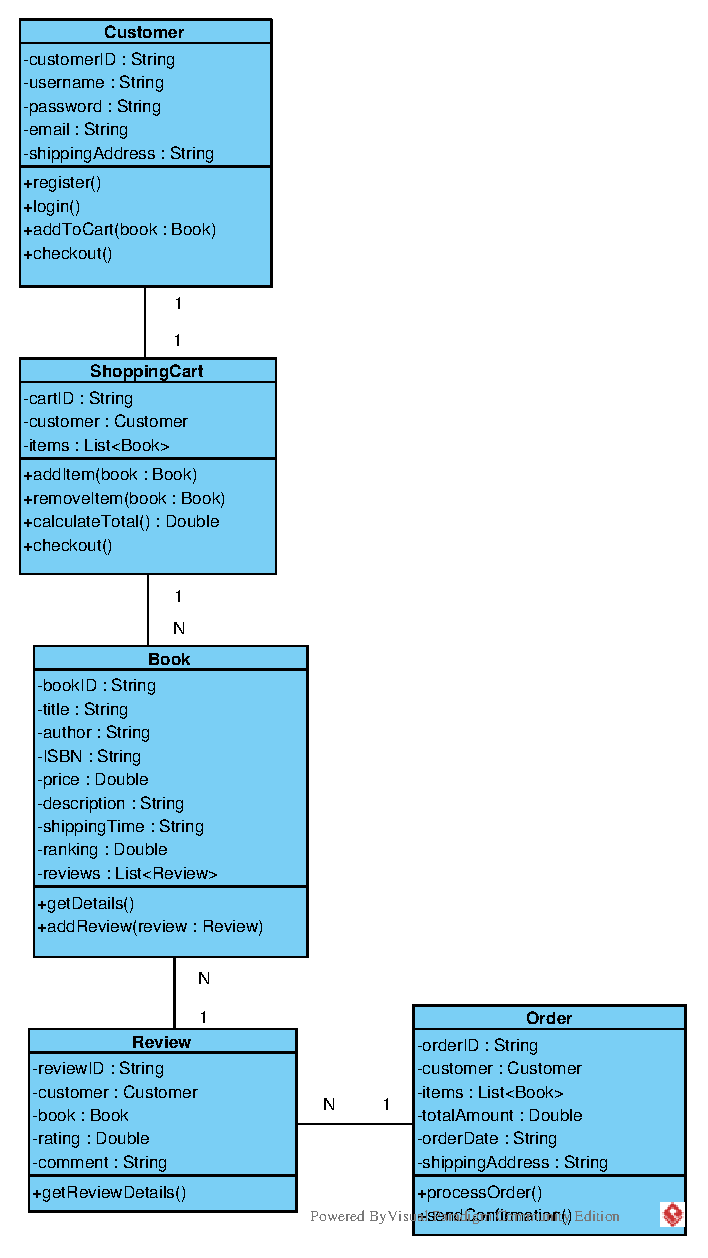
\includegraphics[width=\textwidth]{images/EPS/q6-part2.eps}
    \caption{Class Diagram for E-Bookstore}
    \label{fig:q6-part2}
\end{figure}

\vspace{1em} % Adds space between figures
\begin{figure}[H]
    \centering
    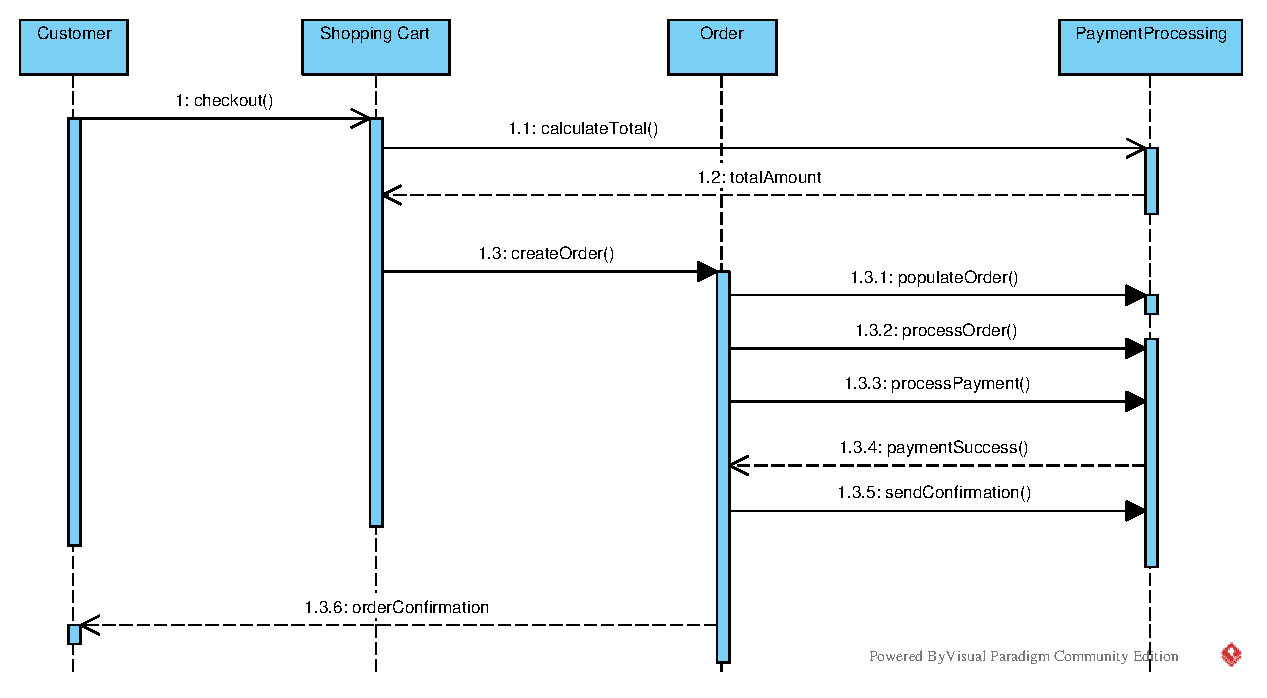
\includegraphics[width=\textwidth]{images/EPS/q6-part3.eps}
    \caption{Sequence Diagram for Checkout Function}
    \label{fig:q6-part3}
\end{figure}

\noindent\rule{\textwidth}{0.4pt} % Line

\vspace{1em} % 
